%%%%% USEFUL MACROS
%
% PROBABILITY
% Expectation:  \E
% Probability:  \Pr
% Variance:     \Var
% KL Div:       \Div{}{}        % looks like D( - || - )
%
% LINEAR ALGEBRA
% Matrix (bf):  \mat{}
% Vector (bf):  \vec{}
%
% ANALYSIS
% Abs:          \abs{}
% Norm:         \norm{}
% Inner prod:   \ip{}
% Argmin:       \argmin{}
% Argmax:       \argmax{}
% Varepsilon:   \eps
%
% COMMON SETS
% Reals:        \bbR
% Rationals:    \bbQ
% Naturals:     \bbN
% Complex Num:  \bbC
% Integers:     \bbZ
% Finite field: \bbF

% Contributors: Vincent Liu, Yadin Rozov, Laura Tinsi
Unsupervised learning begins with the assumption that given a dataset
$\mathcal{X}$, there exists an underlying structure. Our learning task
is to discover this structure given a relatively small amount of data.
One of the most intuitive concepts of a structure is a
cluster---groups of points that behave similarly to each other, but
quite differently to points in other clusters.

To warm up, we can ask a few questions:
\begin{itemize}
\item \emph{What is clustering?} Given input
  data, a clustering algorithm partitions the data into multiple
  `meaningful' groups. 
\item \emph{Why do we need it?} If we can cluster similar points
  together, we can approximate large/infinite/continuous set of
  objects with a finite set of representatives.
\item \emph{What are its applications?} Briefly, applications include
  vector quantization, codebook learning, dictionary learning. It is
  also used in computer vision to map from pixel space to HOG
  (histogram of oriented gradient) space to give rise to new
  features.
\end{itemize}
In short, clustering aims to find a meaningful way to group
datapoints, which is especially important in exploratory data
analysis, helping us understand and summarize input data.


\section{Metric space preliminaries}
\begin{definition}[Metric space]
Let $\mathcal{X}$ be a space and $\rho: \mathcal{X} \times \mathcal{X}
\to \mathbb{R}$ a function. A \emph{metric space} is a pair
$(\mathcal{X},\rho)$ such that $\rho$ satisfies the following:
\begin{itemize}
\item non-negativity (reflexivity): $\forall x,y \in \mathcal{X},
  \rho(x,y) \ge 0$ with equality iff $x=y$ 
\item symmetry: $\forall x,y \in \mathcal{X}, \rho(x,y) = \rho(y,x)$ 
\item triangle inequality: $\forall x,y,z \in \mathcal{X}, \rho(x,y)
  \le \rho(x,z) + \rho(z,y)$. 
\end{itemize}
We call $\rho$ a \emph{metric} or a \emph{distance function}. 
\end{definition}
Given a metric space $\mathcal{X}$, we can define the distance between
a point and a subset $T$ of $\mathcal{X}$: 
\begin{definition}
For a set $T \subset \mathcal{X}$, we define: 
\[\rho(s,T) := \inf_{t\in T} \rho(s,t)\]
\end{definition}

\begin{example} Let $\mathcal{X} = \mathbb{R}^d$. Here are a few
familiar metrics on $\mathcal{X}$:
\begin{itemize}
\item $\ell_2$ distance on $\mathbb{R}^d$: $\forall x,y$,
\[\ell_2(x,y) = \rho(x,y) = \sqrt{\sum_{i=1}^d (x_i - y_i)^2}\] 
\item $\ell_1$  distance on $\mathbb{R}^d$: $\forall x,y$, 
\[\ell_1(x,y) = \rho(x,y) = \sum_{i=1}^d |x_i - y_i|\]
\item $\ell_\infty$ distance on $\mathbb{R}^d$: 
\[\ell_{\infty} = \max_i |x_i - y_i|\]
\end{itemize}
\end{example}

\begin{example}[Geodesics] In a nonlinear space (i.e. a manifold),
the distance between two points is defined as the shortest path
between those two points. If the manifold may be embedded into a
Euclidean space, note that the shortest path on the manifold may
not leave the manifold. We also called this path the shortest 
geodesic.
\end{example}
\begin{figure}
    \centering
    \captionsetup{width=0.8\textwidth}
    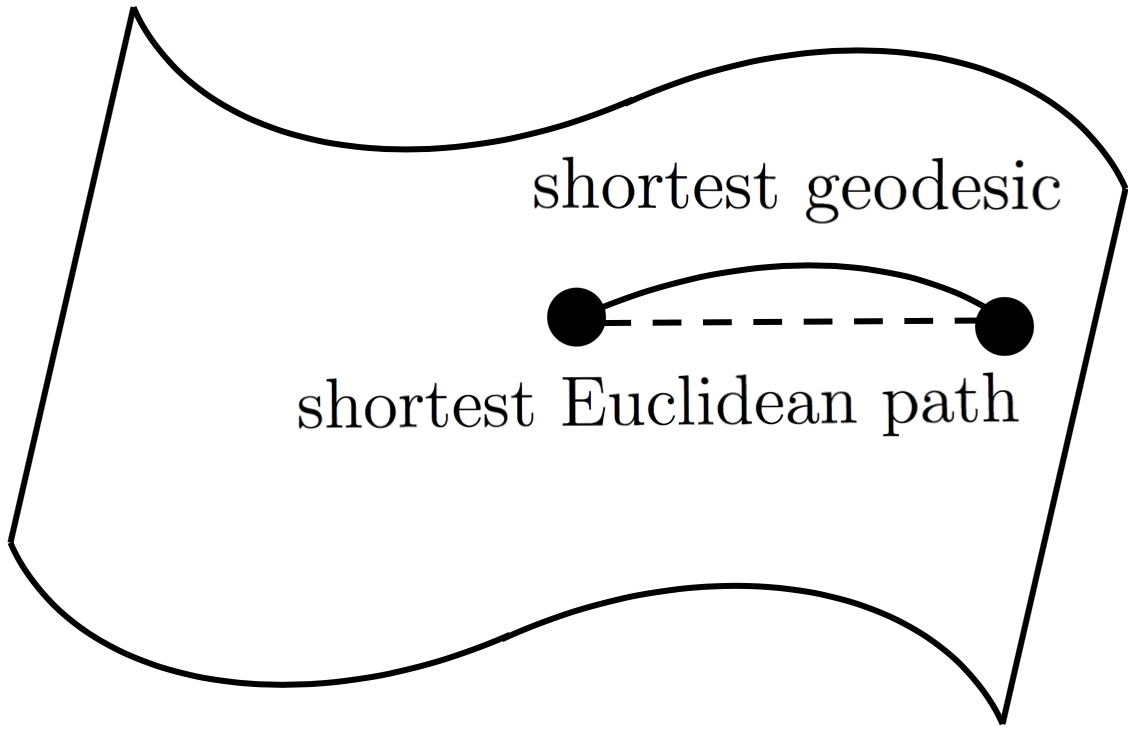
\includegraphics[scale=0.15]{chapter_1/files/geodesic.jpg}
    \caption{A manifold $\mathcal{M}$ embedded in some Euclidean
    space $\mathbb{R}^n$ may have a shortest geodesic that is
    not the same as the shortest Euclidean path.}
    \label{fig:geodesic}
\end{figure}
\begin{example}[Graph metric] The shortest path on graphs (for 
example a social network graph) forms a valid distance function. The
distance is just the smallest number of edges between two vertices.
\end{example}
\begin{remark}
A metric space isn't always a Euclidean space. So, we cannot always
perform Euclidean operations (ie. taking the mean) in an arbitrary
metric space.
\end{remark}

A metric gives a space a notion of distance or similarity. A natural
concept of a \emph{covering} helps us give a space a notion of size.

\begin{definition}[Cover]
Let $S \subset \mathcal{X}$, $\epsilon \geq 0$. A set $T \subset
\mathcal{X}$ is an $\epsilon$-cover of $S$ if:  $\forall s \in S$,
$\exists t \in T$ s.t. $\rho(s,t) \le \epsilon$.
\end{definition}

In other words, $T$ $\epsilon$-covers $S$ if $\sup_{s\in S} 
\rho(s,T)\leq \epsilon$.

\begin{exercise}
(i) Is $S$ a cover of $S$? (ii) Give the vertices $d$-dimensional
cube $\{-1,1\}^d$ the $\ell_\infty$ distance. What is a good 1-cover?
$\frac{1}{2}$-cover? $\frac{9}{10}$-cover?
\end{exercise}

